\documentclass[a4paper,handout,mathserif,final,xcolor=dvipsnames,twocolumn]{beamer}

\useinnertheme{rectangles}
%\useoutertheme{infolines}
\usecolortheme{orchid}
\usetheme{Darmstadt}
\setbeamertemplate{blocks}[rounded][shadow=true]


\usepackage[utf8]{inputenc}
\usepackage{rotating}
\usepackage{multicol}
\usepackage{pstricks}
\usepackage{pst-node}
\usepackage{pst-plot}
\usepackage{amsmath}
%\renewcommand{\bibsection}{\subsubsection*{\bibname } }
\usepackage{natbib}

\newtheorem{thm}{Theorem}[section]
\newtheorem{cor}[thm]{Corollary}
\newtheorem{proposition}[thm]{Proposition}
\newtheorem{condition}[thm]{Buchanan}



\title{Electoral spillovers in Argentina [an attempt at an early draft]}
\author{S. Freille \and  L. Gonzalez  \and M. Nazareno}
% \institute{\inst{1} Unidad Asociada al CONICET - Universidad Católica
%   de Córdoba }}
\date{02 July 2015}

\usepackage{epigraph}

\begin{document}
\maketitle

%\section{Dinero, elecciones y políticas}



\section{Motivationn}
\begin{frame}\frametitle{Correlations}
  \begin{figure}[htbp]
    \centering
    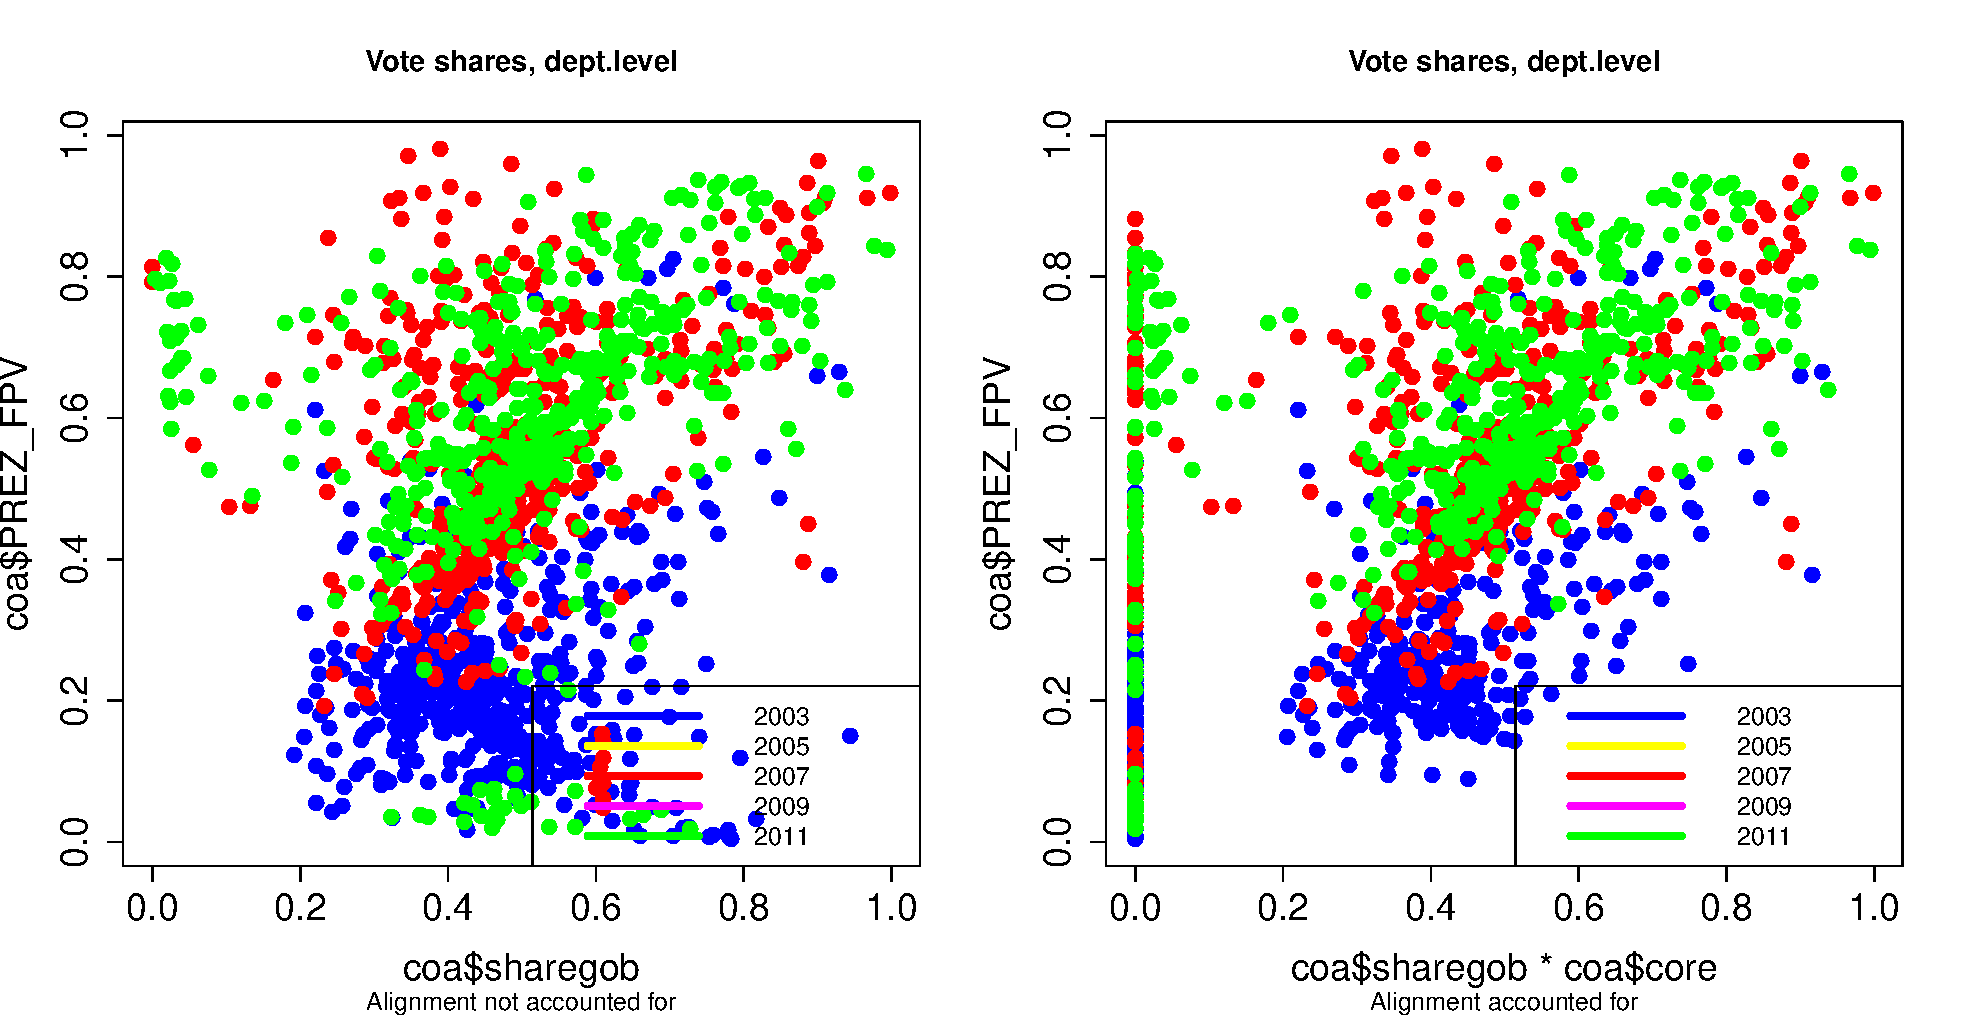
\includegraphics[scale=0.34]{int1}
    \caption{Correlation of vote shares (vertical)}
    \label{fig:1}
  \end{figure}
\end{frame}


\begin{frame}\frametitle{Correlaciones votos (cont.)}
  \begin{figure}[htbp]
    \centering
    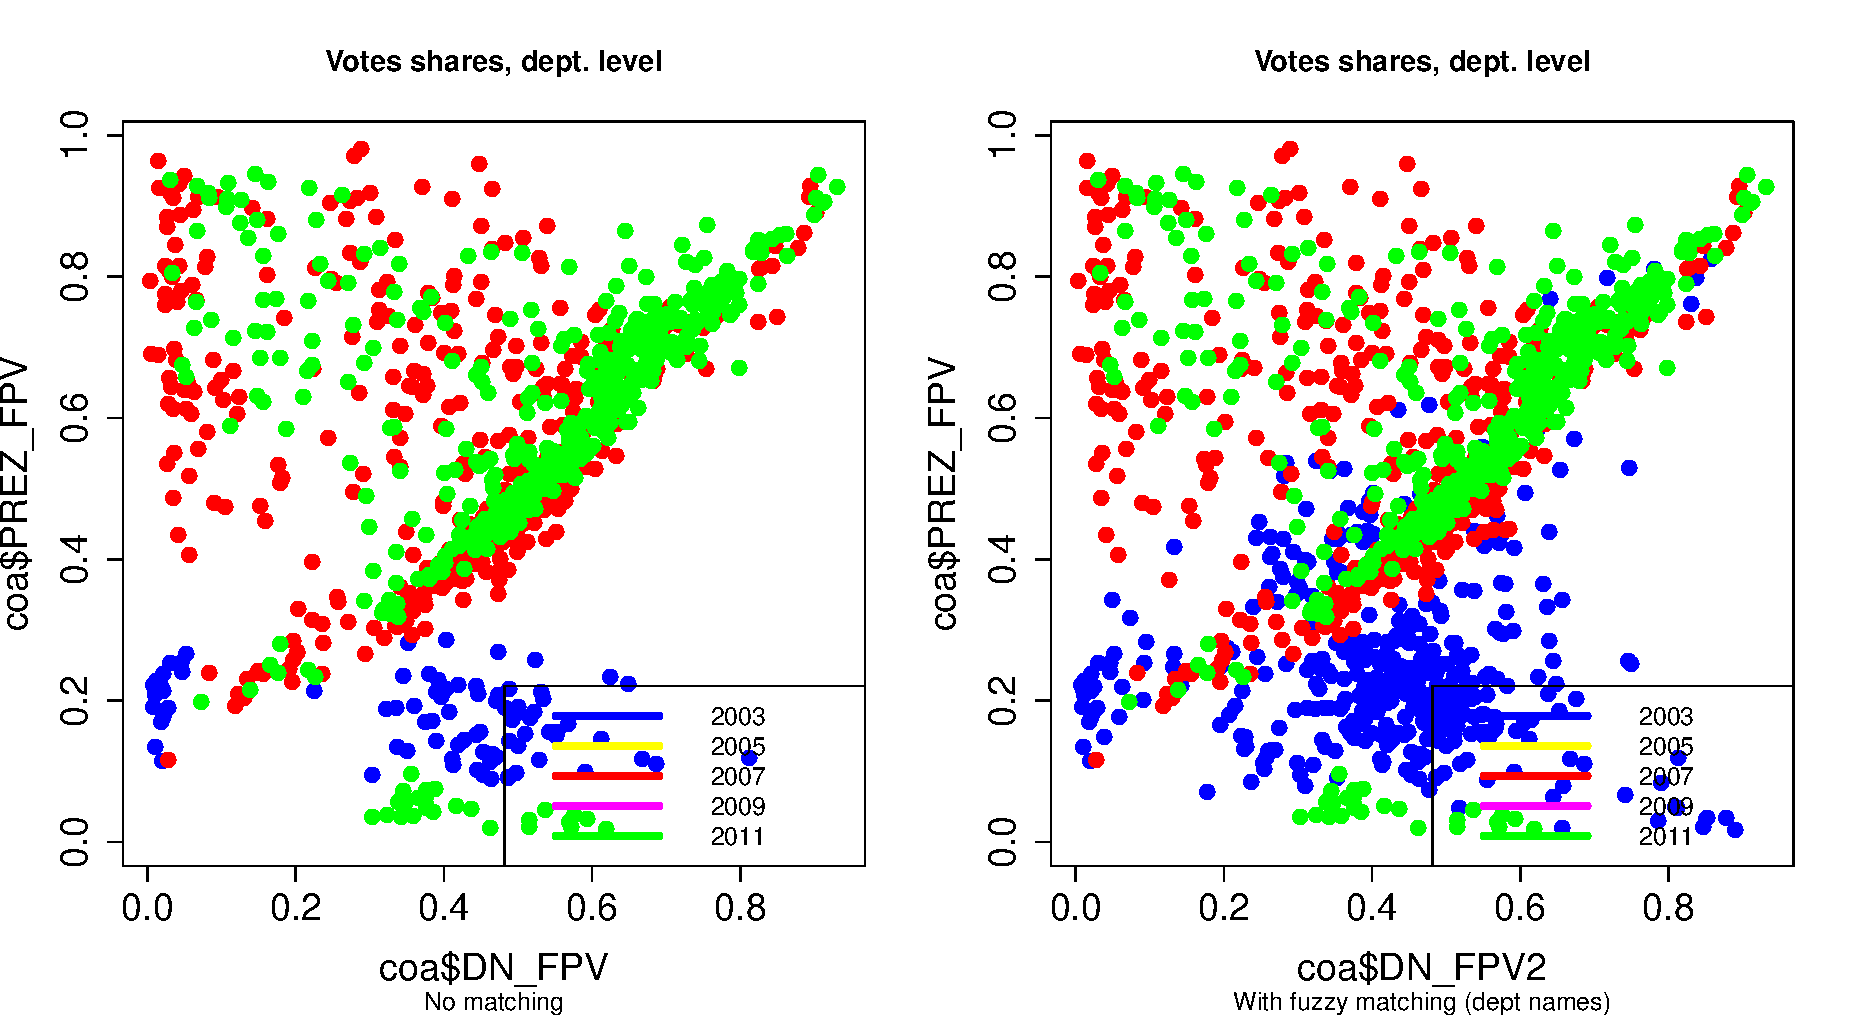
\includegraphics[scale=0.34]{int2}
    \caption{Correlation of vote shares (vertical)}
    \label{fig:1}
  \end{figure}
\end{frame}


\begin{frame}\frametitle{Background}
\begin{itemize}\itemsep 15pt
\item Multi-tiered systems elect representatives at different
levels of government and these elections may be concurrent or
separate.
\item If elected concurrently, a candidate for a given office may
  benefit from electoral spillovers arising from votes received by a
  same-party candidate in another election (\textit{coattail effect})
\item If elected separately, electoral spillovers are still relevant?
\begin{itemize}\itemsep 15pt
\item Two cases: a) lower-level elec \textit{after} upper-level elec;
  b) lower-level elec \textit{before} upper-level elec
\end{itemize}
\end{itemize}
\end{frame}


\begin{frame}\frametitle{Where the literature stands}
\begin{itemize}\itemsep 15pt
\item  Early work studied these electoral effects [\cite{calvert1983},
\cite{ferejohn1984}, \cite{ames1994}, \cite{shugart1995}]
\item More recent work has looked at more rigorous modelling of
  coattail effects  \cite{samuels2000},
\cite{hogan2005}, \cite{oliveros}, \cite{magar2012}, \cite{meredith2013}]
\end{itemize}
\end{frame}

\section{Theory and modelling}
\begin{frame}\frametitle{Some theoretical considerations}
\begin{itemize}\itemsep 15pt
\item Why do these effects arise?:
\begin{itemize} \itemsep 15pt
\item Due to institutional design $\longrightarrow$ ballot designs
  that include a straight-ticket voting may induce larger spillovers
  (coattails)
\item Due to mobilization of party supporters $\longrightarrow$
  particularly relevant in separate elections \cite{meredith2013}
\item Due nationalization/congruence of party system $\longrightarrow$
  homogeneous votes across parties for different elections
\end{itemize}
\end{itemize}
\end{frame}


\begin{frame}\frametitle{Modeling}
\begin{itemize}\itemsep 15pt
\item We follow \cite{shugart1995} in modeling a delayed effect
$\longrightarrow$ only a empirical question [Theory is unclear, both
arguments are likely]
\item Controlling for this is possible and desirable in Argentina
  $\longrightarrow$ normally the delay between elections is less than
  6 months [average distance over three elections equals 80 days]
\item Including a variable measuring for distance between different
  elections makes sense to capture this effect.
\end{itemize}
\end{frame}


\begin{frame}\frametitle{Modeling (cont.)}
\begin{itemize}\itemsep 15pt
\item Assume that there are $n$ sub-national autonomous districts and $one$
  national government. The national government sets the election date
  exogenously. Each subnational government decides upon the date of
  election which can be: 1) before; 2) on the same date; 3) after the
  national date.
\item The decision depends on two factors: 1) the observed intra-party
  ``vertical'' vote deficit in the previous election; 2) the observed
  inter-party district-level margin of victory.
\item The timing of the game is as follows: 1) NatGov chooses elec
  date; 2) each LocGov sets its own elec date; 3) all elections take
  place; 4) each government gets payoff.
\end{itemize}
\end{frame}


\section{Data and results}

\begin{frame}

% Table created by stargazer v.5.1 by Marek Hlavac, Harvard University. E-mail: hlavac at fas.harvard.edu
% Date and time: vie, ago 14, 2015 - 03:08:39 a.m.
% Requires LaTeX packages: dcolumn
\begin{table}[!htbp] \centering
\renewcommand{\arraystretch}{0.8}
\scriptsize
\begin{tabular}{@{\extracolsep{5pt}}lcccc}
\\[-1.8ex]\hline
 & \multicolumn{4}{c}{\textit{Dependent variable: Presidential Vote
   Share [Pooled OLS]}} \\
\cline{2-5} \\
 shgob & -0.87^{***} & -0.80^{***} & -0.07^{**} & -0.46^{***} \\
  & (0.05) & (0.05) & (0.03) & (0.05) \\
 core & -0.26^{***} & -0.21^{***} &  & -0.02 \\
  & (0.03) & (0.03) &  & (0.03) \\
 ENCPrez & -0.11^{***} & -0.11^{***} & -0.10^{***} & -0.09^{***} \\
  & (0.002) & (0.002) & (0.004) & (0.003) \\
 conc &  & -0.07 & -0.11^{**} & 0.54^{***} \\
  &  & (0.04) & (0.06) & (0.07) \\
\textcolor{blue}{days} &  & -0.0004 & -0.03^{***} & -0.03^{***} \\
  &  & (0.01) & (0.01) & (0.01) \\
  shgob:core & 1.00^{***} & 0.86^{***} &  & 0.45^{***} \\
  & (0.05) & (0.05) &  & (0.06) \\
 shgob:conc &  & 0.12^{**} &  & -1.26^{***} \\
  &  & (0.05) &  & (0.12) \\
 core:conc &  &  &  & -0.83^{***} \\
  &  &  &  & (0.07) \\
\textcolor{blue}{shgob:core:conc} &  &  &  & 1.56^{***} \\
  &  &  &  & (0.13) \\
 pubemp &  &  & 0.003^{***} & 0.003^{***} \\
  &  &  & (0.0003) & (0.0002) \\
  conc:shgob &  &  & 0.05 &  \\
  &  &  & (0.06) &  \\
\hline
Observations & \multicolumn{1}{c}{1,390} & \multicolumn{1}{c}{1,301} & \multicolumn{1}{c}{1,240} & \multicolumn{1}{c}{1,240} \\
Adjusted R$^{2}$ & \multicolumn{1}{c}{0.74} & \multicolumn{1}{c}{0.76} & \multicolumn{1}{c}{0.66} & \multicolumn{1}{c}{0.81} \\
F Statistic & \multicolumn{1}{c}{1,010.10$^{***}$} & \multicolumn{1}{c}{596.12$^{***}$} & \multicolumn{1}{c}{395.51$^{***}$} & \multicolumn{1}{c}{545.26$^{***}$} \\
\hline
\textit{Note:}  & \multicolumn{4}{r}{$^{*}$p$<$0.1; $^{**}$p$<$0.05; $^{***}$p$<$0.01} \\
\end{tabular}
\end{table}
\end{frame}



\begin{frame}

% Table created by stargazer v.5.1 by Marek Hlavac, Harvard University. E-mail: hlavac at fas.harvard.edu
% Date and time: vie, ago 14, 2015 - 02:18:37 a.m.
\begin{table}[!htbp] \centering
\renewcommand{\arraystretch}{0.8}
\scriptsize
\begin{tabular}{@{\extracolsep{5pt}}lcccc}
\\[-1.8ex]\hline
\hline \\[-1.8ex]
 & \multicolumn{4}{c}{\textit{Dependent variable: Presidential Vote
   Share [Panel FE, time effects]}} \\
\cline{2-5}
\hline \\[-1.8ex]
 shgob & -0.77^{***} & -0.79^{***} & -1.17^{***} & -0.44^{***} \\
  & (0.07) & (0.05) & (0.09) & (0.05) \\
 core & -0.23^{***} & -0.25^{***} & -0.41^{***} & -0.02 \\
  & (0.03) & (0.03) & (0.05) & (0.03) \\
 conc &  &  &  & 0.54^{***} \\
  &  &  &  & (0.07) \\
 ENCPrez & -0.10^{***} & -0.09^{***} & -0.17^{***} & -0.09^{***} \\
  & (0.003) & (0.003) & (0.01) & (0.003) \\
 PREZ\_FPV\_pre &  &  & 0.26^{***} &  \\
  &  &  & (0.04) &  \\
 \textcolor{blue}{days} &  &  &  & -0.03^{***} \\
  &  &  &  & (0.01) \\
 pubemp &  &  &  & 0.003^{***} \\
  &  &  &  & (0.0002) \\
 shgob:core & 1.00^{***} & 0.94^{***} & 1.19^{***} & 0.44^{***} \\
  & (0.07) & (0.05) & (0.09) & (0.06) \\
 shgob:conc &  &  &  & -1.20^{***} \\
  &  &  &  & (0.12) \\
 core:conc &  &  &  & -0.82^{***} \\
  &  &  &  & (0.07) \\
\textcolor{blue}{shgob:core:conc} &  &  &  & 1.53^{***} \\
  &  &  &  & (0.13) \\
 \hline \\[-1.8ex]
Observations & \multicolumn{1}{c}{1,390} & \multicolumn{1}{c}{1,390} & \multicolumn{1}{c}{357} & \multicolumn{1}{c}{1,240} \\
Adjusted R$^{2}$ & \multicolumn{1}{c}{0.49} & \multicolumn{1}{c}{0.54} & \multicolumn{1}{c}{0.80} & \multicolumn{1}{c}{0.64} \\
F Statistic & \multicolumn{1}{c}{684.62$^{***}$} & \multicolumn{1}{c}{416.90$^{***}$} & \multicolumn{1}{c}{309.84$^{***}$} & \multicolumn{1}{c}{228.07$^{***}$} \\
\hline
\hline \\[-1.8ex]
\textit{Note:}  & \multicolumn{4}{r}{$^{*}$p$<$0.1; $^{**}$p$<$0.05; $^{***}$p$<$0.01} \\
\end{tabular}
\end{table}

\end{frame}

\bibliography{biblio}
\bibliographystyle{plainnat}

\end{document}


\subsection{Actualidad}
\begin{frame}\frametitle{Algunos números}
\begin{itemize}\itemsep 15pt
\item Alrededor de un cuarto de los países democráticos no designan
  una institución formal a cargo de supervisar y controlar los
  informes de los partidos.
\item 68\% de los países tienen financiamiento público a los partidos,
  el resto sólo tiene financiamiento privado (regulado o no) [IDEA]
\item En América Latina, las campañas son cada vez más caras --también
  menos transparentes sobre el origen de los recursos
\item En Argentina en particular, se estiman montos de entre 500 a
  1000 millones para los principales candidatos
\end{itemize}
\end{frame}

\subsection{Relevancia}
\begin{frame}\frametitle{¿Por qué estudiar financiamiento político?}
\begin{itemize}\itemsep 15pt
\item Analizar y explicitar las relaciones entre la forma de
  financiamiento y sus efectos --económicos y políticos-- tema central
  de la economía política
\item Diseño institucional (legal) $\longrightarrow$ puede no ser neutral y
  favorecer a partidos grandes y disminuir niveles de transparencia.
\item Permite aproximarse de manera más sistemática a un aspecto
  central de la corrupción política
\end{itemize}
\end{frame}


\subsection{Contribuciones}
\begin{frame}\frametitle{Contribuciones del trabajo}
\begin{itemize}\itemsep 15pt
\item Entre los primeros análisis empíricos utilizando micro-datos
  para analizar la relación entre dinero y política para Argentina
\item Caracterización teórica del caso de financiamiento mixto
  $\longrightarrow$ lo que importa es el ratio entre contribuciones
  privadas y públicas: mayor el ratio, mayor la proporción de votos
\item Intuición derivada $\longrightarrow$ \textit{incumbents} tienden
  a financiarse por canales no formale para incrementar su
  ventaja. Implicancias para el diseño institucional.
\end{itemize}
\end{frame}

\section{Teoría}
\subsection{Fundamentos teóricos}
\begin{frame}\frametitle{Financiamiento y competencia electoral}
\begin{itemize}\itemsep 15pt\item Financiamiento privado $\longrightarrow$ propuestas de políticas
  de partidos (candidatos) alineados con intereses específicos
  --i.e. alejados del mediano
\item Financiamiento público $\longrightarrow$ propuestas de políticas
  de partidos (candidatos) no alineados con ningún interés particular
  --i.e. coincidentes con el mediano
\item Las existencia de ambos tipos de financiamiento provoca fuerzas
  opuestas en el posicionamiento de las políticas.
\item Si definimos $CEPP=\frac{pri_{i,t}}{pub_{i,t}}$, entonces
  mientras mayor sea este ratio, mayor será la polarización en las
  políticas.
\end{itemize}
\end{frame}

\begin{frame}\frametitle{Financiamiento y competencia electoral (cont.)}
\begin{itemize}\itemsep 10pt
\item El tipo de financiamiento tambien puede estar relacionado con los votos
  obtenidos por los partidos. Dos casos:
\begin{itemize}\itemsep 15pt
\item Partidos simétricos ($p_1=p_2$) $\longrightarrow$ votos son independientes
  de contribuciones e iguales
\item Partidos no simétricos ($p_1 \neq p_2$) $\longrightarrow$ votos
  no son independientes de contribuciones --ejemplo cuando uno es el
  \textit{incumbent} y el otro es el \textit{challenger}.
\end{itemize}
\item Si el gasto en campaña influye sobre la popularidad de los
  partidos esto implicará diferentes porcentajes de votos para
  \textit{incumbents} y \textit{challengers}.
\item Esta diferencia (ventaja del oficialista)
  pareciera estar relacionada
  inversamente con el ratio  $CEPP=\frac{pri_{i,t}}{pub_{i,t}}$.
\end{itemize}
\end{frame}

\subsection{Predicciones}
\begin{frame}\frametitle{Implicancias teóricas y predicciones}
Estas aproximaciones téoricas dan lugar a tres hipótesis testeables: \bigskip
\begin{itemize} \itemsep 15pt
\item Mayor $CEPP=\frac{pri_{i,t}}{pub_{i,t}}$ está asociado a mayor
  polarización en políticas;
\item Menor  $CEPP=\frac{pri_{i,t}}{pub_{i,t}}$. está asociado a mayor
  ventaja del \textit{incumbent} (dado que estos tiene fuentes
  alternativas de financiamiento)
\item Mayores regulaciones (mayores prohibiciones y límites) podrían
  estar asociados a mayor ventaja del \textit{incumbent} (dado que
  podrían limitar la principal fuente de financiamiento de los
  \textit{challengers}).
\end{itemize}
\end{frame}

\subsection{Literatura}


\begin{frame}\frametitle{Literatura relevante}
La literatura es bastante amplia y variada. Entre los principales
referencias se encuentran:
\begin{itemize}\itemsep 15pt
\item Trabajos que estudian el impacto de contribuciones privadas
  sobre los resultados electorales para sistemas bipartidistas y
  distritos de miembro único: Jacobson (1985); Abramowitz (1988); Chappell (1982); Palda
  (1998); Green and Krasno (1988); Stratmann (1991); Gerber (1998); Moon (2002);
\item Trabajos que se enfocan en el caso Argentino $\longrightarrow$
  Ferreira Rubio (2006, 2007); Arrascada y Alonso (2001); De Luca
  (2008).
\item Trabajos que estudian el efecto de reformas en el diseño
  institucional $\longrightarrow$ Che and Gale (1998); Riezman and
  Wilson (1997); Drazen et al (2007).
\end{itemize}
\end{frame}

\section{Diseño Institucional}
\subsection{El caso Argentino}

\begin{frame}\frametitle{Financiamiento político en Argentina}
\begin{itemize}\itemsep 15pt
\item Partidos pueden recibir fondos públicos --suma fija para
  impresión de boletas más suma variable en función de votos previos-
  y fondos privados.
\item Hasta 2009, los partidos podían recibir fondos de
  personas y empresas. La ley 26571 prohibió aportes de empresas.
\item El régimen fue modificado tres veces
  durante el período 2003-2013. Los cambios mas relevantes fueron la
  prohibición de aportes de empresas, y la introducción de de tope de
  aportes de individuos y tope de gastos de campaña.
\end{itemize}
\end{frame}

% \begin{frame}\frametitle{Implicancias}
% \begin{itemize}\itemsep 15pt
% \item El régimen vigente esta potencialmente sesgado en favor de los
%   partidos más grandes, tanto por el aporte público variable como por
%   la posibilidad de recibir de privados.
% \item Para 2013, las contribuciones públicas a los tres principales
%   partidos representaron el 30\% del total de todos los partidos (88
%   en total).
% \item Mientras que las contribuciones privadas a esos mismos tres
%   partidos representaron el 70\% del total de todos los partidos (60
%   partidos).
% \end{itemize}
% \end{frame}


\begin{frame}\frametitle{Composición de fuentes de financiamiento electoral}
\begin{table}\centering\caption{Structure of campaign contributions:
    Argentina,2005-2013} \label{tab:struc1}
\begin{tabular}[htbp]{lcccccc}
  Source & 2005 & 2007 & 2009 & 2011 & 2013 & Period avg \\ \hline\hline
Public & 0.48 & 0.77 & 0.69 & 0.87 & 0.77 & 0.72 \\
Private & 0.23 & 0.17 & 0.27 & 0.12 & 0.20 &  0.20 \\
Other & 0.29 & 0.06 & 0.04 & 0.01 & 0.03 & 0.08 \\ \hline
Total & 1.00 & 1.00 & 1.00 & 1.00 & 1.00 & 1.00 \\
\end{tabular}
\end{table}
\end{frame}

\begin{frame}\frametitle{Limitaciones (disclaimer)}
\begin{itemize}\itemsep 15pt
\item En este trabajo sólo consideramos financiamiento pre-electoral (campañas)

\item Sólo consideramos explícitamente una de las fuentes de
  financiamiento electoral $\longrightarrow$ financiamiento formal
  registrado. Otras dos fuentes posibles:
\begin{itemize}
\item Financiamiento no formal no registrado
\item Financiamiento ilegal
\end{itemize}
\item Estructura de datos no de panel: muy desbalanceado,
  multi-dimension. N muy grande, T pequeño, efectos fijos a nivel
  partido no sensible.
\end{itemize}
\end{frame}


\section{Datos y Metodología}
\subsection{Datos}

\begin{frame}
\begin{itemize}\itemsep 15pt
\item Los datos provienen de diferentes fuentes: a) financiamiento
  político de informes de CNE, de Poder Ciudadano y de la Ruta
  Electoral; b) datos electorales del Ministerio del Interior, la CNE
  y complementados con el Atlas Electoral de Andy Tow.
\item Los datos cubren solamente elecciones para cargos nacionales
  (incluyendo primarias)
  --Presidente, DN y SN-- para todos los años entre 2005 y 2013.
\item Los micro-datos al nivel del individuo --aporte del invididuo
  ``i'' al partido ``j'' en distrito ``k'' fueron agregados al nivel
  del partido y/o alianza.
\item Numerosos inconvenientes: a) variación del nro de
  partidos por distrito enre elecciones; b) party-y/o-alianza para
  maximizar casos.
\end{itemize}
\end{frame}


% \begin{frame}


% \begin{table}[htbp]
%   \centering
%  \caption{Parties/alliances by election type and elective office}
%   \label{tab:descr1}
% \begin{scriptsize}
%   \begin{tabular}[htbp]{lccccccccc}
%     \textbf{office} & \textbf{General} &  &  & &  & \textbf{Primary}  & & & &  \\
%     \hline\hline
%   &  \textit{2005} &  \textit{2007} & \textit{2009} & \textit{2011} & \textit{2013} & \textit{Total}  & \textit{2011} & \textit{2013} & \textit{Total} \\
% Dip (LH) & 181 & 339 & 271 & 154 & 140 & 1085 & 203 & 173 & 376 \\
% Pre y Vice &  --  & 385 & -- & 170 & -- & 555 & 240 & -- & 240 \\
% Sen (UH) &  46  &  110 & 101 & 43 & 44 & 344 & 62 & 60 & 122 \\
% \hline\hline
% Total & 227 & 834 & 372 & 367 & 184 & 1984  & 505 & 233 & 738 \\
%   \end{tabular}
% \end{scriptsize}
% \end{table}


% \end{frame}


\subsection{Estadísticas descriptivas}


\begin{frame}\frametitle{Operativización}
\begin{itemize}\itemsep 15pt
\item Tenemos dos alternativas de operativización de la variable
  independiente:
\begin{itemize}\itemsep 10pt
\item Total de contribuciones privadas y públicas [$cpri_c$, $cpub_c$]
\item Ratio de contribuciones privadas sobre contribuciones totales
  [$cpubt$, $cprit$, $cpripub$]
\end{itemize}
\item Tratamiento de ceros $\longrightarrow$ de las 2722
  observaciones, 1294 tienen contribuciones públicas positivas y
  sólo 594 tienen contribuciones privadas positivas [1433 obs con
  algún tipo de contribución]. El interés es en
  el ratio $\longrightarrow$ descartamos casos de ambos aportes
  iguales a cero.
\end{itemize}
\end{frame}

\begin{frame}\frametitle{Aportes y votos}
\begin{figure}[htbp]
  \centering
  \includegraphics[scale=0.35]{scatterplot1}
  \caption{Private contributions and vote shares}
  \label{fig:scatterplot1}
\end{figure}
\end{frame}

\begin{frame}\frametitle{Heterogeneidad}
\begin{figure}[htbp]
  \centering
  \includegraphics[scale=0.25]{grafico1}
  \caption{Private funds as fraction of total funds}
  \label{fig:fig1}
\end{figure}
\end{frame}



\begin{frame}\frametitle{Pre y post ley 26571}
\begin{table}[htbp]
  \centering
  \begin{tabular}[htbp]{p{4cm}cccc}
    \textbf{Concept} &	\textbf{2007} &	\textbf{2009}	& \textbf{2011} &	\textbf{2013} \\ \hline\hline
Ratio of private-to-total (full sample) &	0.17 &	0.26 &
0.11 &	0.21 \\
Ratio of private-to-total (positive private contributions) &
0.53 &	0.51 &	0.32 &	0.39 \\
Ratio of non-corporate (personal) to private (full sample) &
0.84 &	0.89 &	1 &	1 \\
  \end{tabular}
  \caption{Structure of party financing pre and after reform}
  \label{tab:tab1}
\end{table}
\end{frame}




\subsection{Especificación}
\begin{frame}\frametitle{Estrategia empírica}
\begin{itemize}\itemsep 15pt
\item Dos variables principales: contribuciones de campaña (VI) y
  porcentaje de votos (VD). Desagregadas por elección, distrito y
  año.
\begin{equation*}
sh_{isht}=\beta_{0}+\beta_{1}pri_{isht}+\beta_{2}comp_{sht}+marginpre_{sht}+\beta_{3}oth_{isht}+\epsilon_{isht}
\end{equation*}
\item  $sh_{isht}$ y $pri_{isht}$ son el porcentaje de votos y el
  monto de contribuciones privadas recibidas por el partido/alianza
  $i$ en el distrito $s$ en la elección $h$ para el año $t$. $comp$ y
  $marginpre$ variables de control.
\end{itemize}
\end{frame}


\section{Resultados}

\subsection{Salidas}

\begin{frame}
% Table created by stargazer v.5.1 by Marek Hlavac, Harvard University. E-mail: hlavac at fas.harvard.edu
% Date and time: mar, jun 09, 2015 - 19:08:15
\renewcommand{\arraystretch{0.7}}

\begin{table}[!h] \centering
\scriptsize
\begin{tabular}{@{\extracolsep{0pt}}lp{1cm}p{1cm}p{1cm}p{1cm}p{1cm}p{1cm}p{1cm}}
\\[-1.8ex]\hline
\hline \\[-1.8ex]
 & \multicolumn{7}{c}{\textit{Dependent variable: sh [Method: Pooled OLS]}} \\
%\cline{2-8}
%\\[-1.8ex] & \multicolumn{7}{c}{sh} \\
\\[-1.8ex] & (1) & (2) & (3) & (4) & (5) & (6) & (7)\\
\hline \\[-1.8ex]
 cpri\_c & 0.00$^{***}$ &  &  &  &  &  &  \\
  & (0.00) &  &  &  &  &  &  \\
  cpub\_c & 0.00$^{***}$ &  &  &  &  &  &  \\
  & (0.00) &  &  &  &  &  &  \\
  cpubt &  & $-$0.08$^{***}$ &  &  &  &  &  \\
  &  & (0.01) &  &  &  &  &  \\
  cprit &  &  & 0.09$^{***}$ & 0.06$^{***}$ &  &  &  \\
  &  &  & (0.01) & (0.01) &  &  &  \\
  l(cpripub) &  &  &  &  & 0.003$^{***}$ & 0.003$^{*}$ & 0.004$^{***}$ \\
  &  &  &  &  & (0.001) & (0.001) & (0.001) \\
  comp & $-$0.01$^{***}$ & $-$0.01$^{***}$ & $-$0.01$^{***}$ & $-$0.004$^{***}$ & $-$0.004$^{***}$ & $-$0.004$^{***}$ & $-$0.004$^{***}$ \\
  & (0.00) & (0.001) & (0.001) & (0.001) & (0.001) & (0.001) & (0.001) \\
  marginpre & 0.09$^{***}$ & 0.09$^{***}$ & 0.10$^{***}$ & 0.004 & $-$0.01 & $-$0.01 & $-$0.01 \\
  & (0.03) & (0.03) & (0.03) & (0.03) & (0.03) & (0.03) & (0.03) \\
  l(.):shpre2 &  &  &  &  &  &  & $-$0.01$^{***}$ \\
  &  &  &  &  &  &  & (0.004) \\
  shpre2 &  &  &  & 0.66$^{***}$ & 0.67$^{***}$ & 0.67$^{***}$ & 0.61$^{***}$ \\
  &  &  &  & (0.02) & (0.02) & (0.02) & (0.03) \\
  l(.):comp &  &  &  &  &  & 0.00 &  \\
  &  &  &  &  &  & (0.00) &  \\
  \hline \\[-1.8ex]
Observations & 1,431 & 1,431 & 1,431 & 911 & 891 & 891 & 891 \\
R$^{2}$ & 0.11 & 0.11 & 0.11 & 0.52 & 0.51 & 0.51 & 0.52 \\
Adjusted R$^{2}$ & 0.10 & 0.11 & 0.11 & 0.52 & 0.51 & 0.51 & 0.51 \\
F Statistic & 42.1$^{***}$ & 57.8$^{***}$ & 60.7$^{***}$ & 243$^{***}$ & 233$^{***}$ & 186$^{***}$ & 189$^{***}$ \\
\hline
\hline \\[-1.8ex]
\textit{Note:}  & \multicolumn{7}{r}{$^{*}$p$<$0.1; $^{**}$p$<$0.05; $^{***}$p$<$0.01} \\
\end{tabular}
\end{table}
\end{frame}

\begin{frame}\frametitle{Salidas (cont.)}
\begin{itemize}\itemsep 10pt
\item Modelo 1 incluye totales; 2 a 4 ratio sobre totales; 5 a 7
  ratio privado/público. El signo esperado para los coeficientes de
  $cpri_c$, $cprit$ y $cpripub$ es positivo; el signo esperado para
  los coeficientes de $cpub_c$, $cpubt$ es positivo.
\item Un incremento de una desviación estandar en las contribuciones
  privadas incrementaría el \textit{vote share} en sólo 0.01.
\item Las variables de control tienen el signo esperado. Una variable
  importante es $shpre2$, el $vote share$ --party-level var-- del partido/alianza en la
  elección correspondiente anterior en el distrito.
\item Evidencia de interacciones
\end{itemize}
\end{frame}


\begin{frame}
% Table created by stargazer v.5.1 by Marek Hlavac, Harvard University. E-mail: hlavac at fas.harvard.edu
% Date and time: mar, jun 09, 2015 - 19:08:59
\renewcommand{\arraystretch{0.7}}
\begin{table}[!h] \centering
\scriptsize
\begin{tabular}{@{\extracolsep{0pt}}lp{1cm}p{1cm}p{1cm}p{1cm}p{1cm}p{1cm}p{1cm}}
\\[-1.8ex]\hline
\hline \\[-1.8ex]
 & \multicolumn{7}{c}{\textit{Dependent variable: sh [Method: Pooled
   OLS (only positive priv contr]}} \\
\\[-1.8ex] & (1) & (2) & (3) & (4) & (5) & (6) & (7)\\
\hline \\[-1.8ex]
 cpri\_c & 0.000$^{*}$ &  &  &  &  &  &  \\
  & (0.00) &  &  &  &  &  &  \\
  cpub\_c & 0.00$^{***}$ &  &  &  &  &  &  \\
  & (0.000) &  &  &  &  &  &  \\
  cpubt &  & $-$0.04$^{**}$ &  &  &  &  &  \\
  &  & (0.02) &  &  &  &  &  \\
  cprit &  &  & 0.04$^{**}$ & 0.04$^{**}$ &  &  &  \\
  &  &  & (0.02) & (0.02) &  &  &  \\
  l(cpripub) &  &  &  &  & 0.0002 & $-$0.001 & 0.002 \\
  &  &  &  &  & (0.001) & (0.003) & (0.002) \\
  comp & $-$0.01$^{***}$ & $-$0.01$^{***}$ & $-$0.01$^{***}$ & $-$0.004$^{***}$ & $-$0.004$^{***}$ & $-$0.004$^{***}$ & $-$0.004$^{***}$ \\
  & (0.001) & (0.001) & (0.001) & (0.001) & (0.001) & (0.001) & (0.001) \\
  marginpre & 0.13$^{***}$ & 0.14$^{***}$ & 0.14$^{***}$ & 0.08$^{*}$ & 0.06 & 0.06 & 0.06 \\
  & (0.04) & (0.04) & (0.04) & (0.04) & (0.04) & (0.04) & (0.04) \\
  l(.):shpre2 &  &  &  &  &  &  & $-$0.01 \\
  &  &  &  &  &  &  & (0.01) \\
  shpre2 &  &  &  & 0.59$^{***}$ & 0.60$^{***}$ & 0.60$^{***}$ & 0.60$^{***}$ \\
  &  &  &  & (0.04) & (0.04) & (0.04) & (0.04) \\
  l(.):comp &  &  &  &  &  & 0.0001 &  \\
  &  &  &  &  &  & (0.0002) &  \\
 Observations & 593 & 593 & 593 & 405 & 405 & 405 & 405 \\
R$^{2}$ & 0.12 & 0.11 & 0.11 & 0.44 & 0.44 & 0.44 & 0.44 \\
Adjusted R$^{2}$ & 0.12 & 0.10 & 0.10 & 0.44 & 0.43 & 0.43 & 0.43 \\
F Statistic & 20.91$^{***}$ & 23.12$^{***}$ & 23.65$^{***}$ & 79.28$^{***}$ & 77.02$^{***}$ & 61.61$^{***}$ & 62.15$^{***}$ \\
\hline
\hline \\[-1.8ex]
\textit{Note:}  & \multicolumn{7}{r}{$^{*}$p$<$0.1; $^{**}$p$<$0.05; $^{***}$p$<$0.01} \\
\end{tabular}
\end{table}
\end{frame}



\begin{frame}\frametitle{Salidas (cont.)}
\begin{itemize}\itemsep 15pt
\item Sólo partidos que han recibido aportes privados. Resultados
  cualitativamnete similares a los anteriores. Sin embargo:
\begin{itemize}
\item Pérdida importante de observaciones
\item La variable $cpripub$ deja de ser significativa en los modelos 5
  a 7 (sample/missing vbles)
\end{itemize}
\item Si tenemos en cuenta la \textit{estructura} de los datos,
  podemos utilizar modelos de efectos mixtos para capturar efectos a
  distinto nivel.
\end{itemize}
\end{frame}


\begin{frame}
% Table created by stargazer v.5.1 by Marek Hlavac, Harvard University. E-mail: hlavac at fas.harvard.edu
% Date and time: Mon, Jun 15, 2015 - 09:11:04 PM
\renewcommand{\arraystretch{0.75}}
\begin{table}[!htbp] \centering

\scriptsize
\begin{tabular}{@{\extracolsep{0pt}}lccccc}
\\[-1.8ex]\hline
\hline \\[-1.8ex]
 & \multicolumn{5}{c}{\textit{Dependent variable: sh [Model: Linear
   Mixed Effects}} \\
\\[-1.8ex] & (1) & (2) & (3) & (4) & (5)\\
\hline \\[-1.8ex]
 cpri\_c & 0.0000$^{**}$ &  &  &  &  \\
  & (0.00) &  &  &  &  \\
  cpub\_c & 0.0000$^{***}$ &  &  &  &  \\
  & (0.0000) &  &  &  &  \\
  cprit &  & 0.06$^{***}$ & 0.07$^{***}$ & 0.07$^{***}$ &  \\
  &  & (0.01) & (0.01) & (0.01) &  \\
  cpripub &  &  &  &  & 0.0000 \\
  &  &  &  &  & (0.0000) \\
  comp & $-$0.01$^{***}$ & $-$0.004$^{***}$ & $-$0.004$^{***}$ & $-$0.004$^{***}$ & $-$0.004$^{***}$ \\
  & (0.001) & (0.001) & (0.001) & (0.001) & (0.001) \\
  marginpre & 0.09$^{***}$ & 0.002 & 0.01 & 0.01 & $-$0.01 \\
  & (0.03) & (0.03) & (0.03) & (0.03) & (0.03) \\
  shpre2 &  & 0.66$^{***}$ & 0.65$^{***}$ & 0.65$^{***}$ & 0.67$^{***}$ \\
  &  & (0.02) & (0.02) & (0.02) & (0.02) \\
 Observations & 1,431 & 911 & 911 & 911 & 891 \\
Akaike Inf. Crit. & $-$1,126.64 & $-$1,172.54 & $-$1,187.92 & $-$1,185.94 & $-$1,125.62 \\
Bayesian Inf. Crit. & $-$1,089.78 & $-$1,138.84 & $-$1,149.40 & $-$1,142.61 & $-$1,087.29 \\
\hline
\hline \\[-1.8ex]
\textit{Note:}  & \multicolumn{5}{r}{$^{*}$p$<$0.1; $^{**}$p$<$0.05; $^{***}$p$<$0.01} \\
\end{tabular}
\end{table}
\end{frame}


\begin{frame}

\begin{table}[!h] \centering

\scriptsize
\begin{tabular}{@{\extracolsep{0pt}}lccccc}
\\[-1.8ex]\hline
\hline \\[-1.8ex]
 & \multicolumn{5}{c}{\textit{Dependent variable: sh [Model: Linear
   Mixed Effects (pos pri]}} \\
\\[-1.8ex] & (1) & (2) & (3) & (4) & (5)\\
\hline \\[-1.8ex]
 cpri\_c & 0.0000$^{*}$ &  &  &  &  \\
  & (0.00) &  &  &  &  \\
  cpub\_c & 0.0000$^{***}$ &  &  &  &  \\
  & (0.0000) &  &  &  &  \\
  cprit &  & 0.04$^{**}$ & 0.04$^{**}$ & 0.04$^{**}$ &  \\
  &  & (0.02) & (0.02) & (0.02) &  \\
  cpripub &  &  &  &  & 0.0000 \\
  &  &  &  &  & (0.0000) \\
  comp & $-$0.01$^{***}$ & $-$0.004$^{***}$ & $-$0.004$^{***}$ & $-$0.004$^{***}$ & $-$0.004$^{***}$ \\
  & (0.001) & (0.001) & (0.001) & (0.001) & (0.001) \\
  marginpre & 0.13$^{***}$ & 0.07 & 0.07 & 0.07 & 0.06 \\
  & (0.04) & (0.04) & (0.04) & (0.04) & (0.04) \\
  shpre2 &  & 0.59$^{***}$ & 0.59$^{***}$ & 0.59$^{***}$ & 0.60$^{***}$ \\
  &  & (0.04) & (0.04) & (0.04) & (0.04) \\
 Observations & 593 & 405 & 405 & 405 & 405 \\
Akaike Inf. Crit. & $-$456.99 & $-$463.17 & $-$461.17 & $-$459.17 & $-$456.13 \\
Bayesian Inf. Crit. & $-$426.29 & $-$435.14 & $-$429.14 & $-$423.14 & $-$424.10 \\
\hline
\hline \\[-1.8ex]
\textit{Note:}  & \multicolumn{5}{r}{$^{*}$p$<$0.1; $^{**}$p$<$0.05; $^{***}$p$<$0.01} \\
\end{tabular}
\end{table}
\end{frame}


\begin{frame}
\begin{itemize}\itemsep 15pt
\item Testeamos por efectos de grupos para: provincias (si); office
  (si) y primaria (no). Los resultados para el modelo de random
  intercepts estan en la figura.
\end{itemize}
\begin{figure}[htbp]
  \centering
  \includegraphics[scale=0.3]{dotplot1}
    \label{fig:dotplot1}
\end{figure}
\end{frame}



\begin{frame}\frametitle{Incumbents vs challengers}
% Table created by stargazer v.5.1 by Marek Hlavac, Harvard University. E-mail: hlavac at fas.harvard.edu
% Date and time: Lun, Jun 15, 2015 - 10:38:08 p.m.
\begin{table}[!h] \centering
\scriptsize
\begin{tabular}{@{\extracolsep{0pt}}lcccc}
\\[-1.8ex]\hline
\hline \\[-1.8ex]
 & \multicolumn{4}{c}{\textit{Dependent variable: sh}} \\
\\[-1.8ex] & Inc & Ch & Inc (RS) & Cha (RS)\\
\hline \\[-1.8ex]
\\[-1.8ex] & (1) & (2) & (3) & (4)\\
\hline \\[-1.8ex]\\
 cprit & $-$0.06$^{*}$ & 0.04$^{***}$ & $-$0.07$^{*}$ & $-$0.01 \\
  & (0.03) & (0.01) & (0.04) & (0.04) \\
  comp & $-$0.01$^{***}$ & $-$0.002$^{***}$ & $-$0.01$^{***}$ & $-$0.001 \\
  & (0.002) & (0.0004) & (0.002) & (0.002) \\
  marginpre & $-$0.03 & 0.02 & 0.06 & 0.13$^{*}$ \\
  & (0.09) & (0.02) & (0.09) & (0.08) \\
  shpre2 & 0.45$^{***}$ & 0.25$^{***}$ & 0.34$^{***}$ & 0.67$^{***}$ \\
  & (0.08) & (0.03) & (0.08) & (0.07) \\
  Constant & 0.32$^{***}$ & 0.06$^{***}$ & 0.32$^{***}$ & 0.05 \\
  & (0.04) & (0.01) & (0.04) & (0.03) \\
 \hline \\[-1.8ex]
Observations & 123 & 265 & 80 & 112 \\
R$^{2}$ & 0.42 & 0.32 & 0.43 & 0.51 \\
Adjusted R$^{2}$ & 0.40 & 0.31 & 0.40 & 0.49 \\
F Statistic & 21.35$^{***}$ & 31.12$^{***}$ & 14.08$^{***}$ & 28.15$^{***}$ \\
\hline
\hline \\[-1.8ex]
\textit{Note:}  & \multicolumn{4}{r}{$^{*}$p$<$0.1; $^{**}$p$<$0.05; $^{***}$p$<$0.01} \\
\end{tabular}
\end{table}
\end{frame}


\begin{frame}
\begin{figure}[htbp]
  \centering
  \includegraphics[scale=0.32]{scatterplots2}
  \caption{Vote shares and private financing: Incumbents vs Challengers}
  \label{fig:scatterplots2}
\end{figure}
\end{frame}


\begin{frame}\frametitle{Resultados (cont.)}
\begin{itemize}\itemsep 15pt
\item Segmentando la muestra para incumbents y challengers, vemos que
  los resultados cambian significativamente.
\item $cprit$ signo positivo para challengers y signo negativo para
  incumbents.
\begin{itemize}
\item La unica explicación razonable que encontramos es que el signo
  negativo para incumbents refleje parte de un efecto sustitución
  asociado a tipos de financiamiento --i.e. formal vs informal.
\item Una forma de capturar esto sería tomar el gasto en publicidad
  oficial del incumbent en tiempos pre-electorales en determinados
  rubros --i.e. TV, cadena nacional, avisos FPT, etc. Aún así, no hay
 a priori una forma de asignar que fracción de ese gasto pueda
 asignarse a campaña.
\end{itemize}
\item Resultados avalan una de nuestras hipótesis.
\end{itemize}
\end{frame}

% \begin{frame}\frametitle{Extensiones y ampliaciones}
% \begin{itemize}\itemsep 15pt
% \item Examinar los determinantes de las contribuciones privadas
%   individuales --personas físicas y jurídicas. Evaluar hipótesis de
%   donantes a la Grossman \& Helpman
% \item Examinar la relación entre aportes privados y políticas
%   aplicadas --votaciones individuales en Congreso según categorización
%   de leyes; indicadores de rentabilidad de empresas y grupos de
%   interés; evidencia de licitaciones y tratamiento diferencial.
% \item Explorar canales informales e ilegales de financiamiento de modo
%   a caracterizar su influencia en el proceso electoral y de formación
%   de políticas.
% \end{itemize}
% \end{frame}


\end{document}

